\documentclass{article}
\usepackage{graphics}
\usepackage{indentfirst}
\usepackage{amsmath}
\usepackage{algorithm}
\usepackage{algorithmic}
\usepackage{bm}
\usepackage{setspace}
\usepackage{graphicx}
\usepackage{float}
\usepackage{CJKutf8}



\title{GAN ZOO}
\author{Ruichen Wang}

\begin{document}
\begin{CJK*}{UTF8}{gbsn}
\maketitle
\begin{abstract}
GAN动物园
\end{abstract}

\tableofcontents
\section{GAN}
最初GAN\cite{DBLP:conf/nips/GoodfellowPMXWOCB14} 是Ian J. Goodfellow 在2014年提出的。
\section{DCGAN}
\noindent
DCGAN \cite{journals/corr/RadfordMC15} 主要优化点: \\
\begin{itemize}
\item 用strided convolutions (也可以称作‘反卷积’) 替换 spatial pooling functions (比如 max pooling)
\item 在generator和discriminator中都使用 batch norm
\item 移除FC hidden layers
\item 除最后output使用tanh以外, generator所有的avtivation都用ReLU
\item 在discriminator所有层中都使用LeakyReLU
\end{itemize}

在图像分类中,使用Global Average Pooling(GAP) 替换 FC 可以取得更好的结果。 论文发现GAP虽然可以提高模型稳定性,但是会减缓收敛速度。采用直接把conv的特征与输出层相连效果也很好。

\begin{figure}[H]
\centering
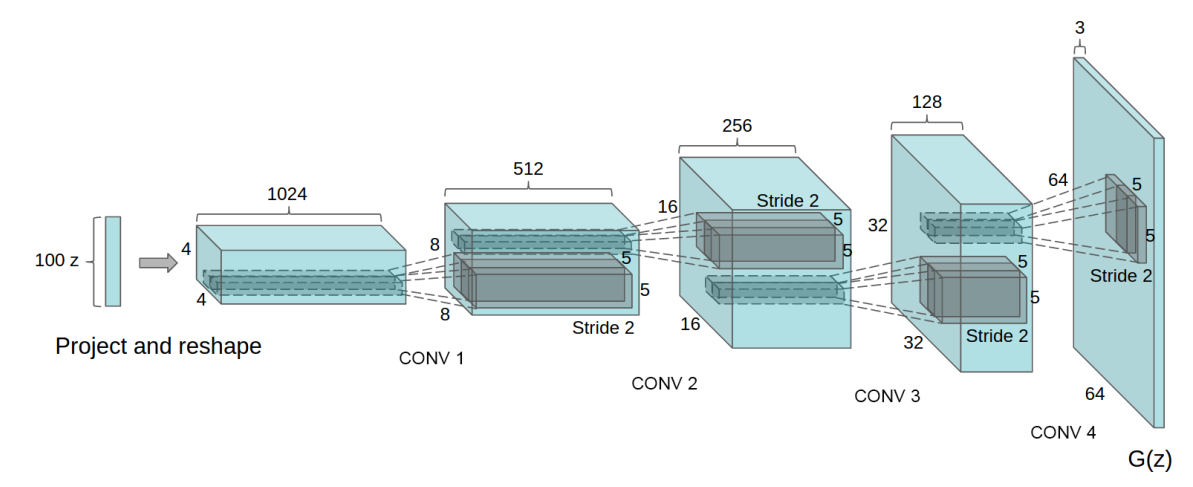
\includegraphics[width=5in,height=2in]{DCGAN}
\caption{DCGAN}
\end{figure}

\bibliographystyle{plain}
\bibliography{ref}

\end{CJK*}
\end{document}




















